\documentclass[compress,red]{beamer}
\usepackage[utf8]{inputenc}
\usepackage{ucs}
\usepackage{amsmath}
\usepackage{amsfonts}
\usepackage{amssymb}
\usepackage[russian]{babel}
\usepackage{graphicx}
\usepackage{wrapfig}

\usepackage{tikz}
\usepackage{verbatim}

\usepackage{color}
\usepackage{xcolor}
\usepackage{listings}

\usepackage{caption}

\lstset{
language=ruby,
extendedchars=\true,
inputencoding=utf8x,
commentstyle=\itshape,
stringstyle=\bf,
belowcaptionskip=5pt }


\DeclareCaptionFont{white}{\color{white}}
\DeclareCaptionFormat{listing}{\colorbox{gray}{\parbox{\textwidth}{#1#2#3}}}
\captionsetup[lstlisting]{format=listing,labelfont=white,textfont=white}

\usetikzlibrary{calc,trees,positioning,arrows,chains,shapes.geometric,%
    decorations.pathreplacing,decorations.pathmorphing,shapes,%
    matrix,shapes.symbols}

\tikzset{
>=stealth',
  punktchain/.style={
    rectangle, 
    rounded corners, 
    % fill=black!10,
    draw=black, very thick,
    text width=10em, 
    minimum height=3em, 
    text centered, 
    on chain},
  line/.style={draw, thick, <-},
  element/.style={
    tape,
    top color=white,
    bottom color=blue!50!black!60!,
    minimum width=8em,
    draw=blue!40!black!90, very thick,
    text width=10em, 
    minimum height=1.5em, 
    text centered, 
    on chain},
  every join/.style={->, thick,shorten <=1pt},
  decoration={brace},
  tuborg/.style={decorate},
  tubnode/.style={midway, right=2pt},
}

\mode<presentation>

\usetheme{Warsaw}

\definecolor{Red}{rgb}{1,0,0}
\definecolor{Blue}{rgb}{0,0,1}
\definecolor{Green}{rgb}{0,1,0}
\definecolor{magenta}{rgb}{1,0,.6}
\definecolor{lightblue}{rgb}{0,.5,1}
\definecolor{lightpurple}{rgb}{.6,.4,1}
\definecolor{gold}{rgb}{.6,.5,0}
\definecolor{orange}{rgb}{1,0.4,0}
\definecolor{hotpink}{rgb}{1,0,0.5}
\definecolor{newcolor2}{rgb}{.5,.3,.5}
\definecolor{newcolor}{rgb}{0,.3,1}
\definecolor{newcolor3}{rgb}{1,0,.35}
\definecolor{darkgreen1}{rgb}{0, .35, 0}
\definecolor{darkgreen}{rgb}{0, .6, 0}
\definecolor{darkred}{rgb}{.75,0,0}

\xdefinecolor{olive}{cmyk}{0.64,0,0.95,0.4}
\xdefinecolor{purpleish}{cmyk}{0.75,0.75,0,0}

\useoutertheme[subsection=false]{smoothbars}

\title{Функции в электронных таблицах}

%\usecolortheme{dolphin}


\begin{document}
%%титульная страница
\maketitle
%% основные моменты

\section{Морской бой}

\subsection{Интервалы}
\begin{frame}[fragile]
  \frametitle{Интервалы}
  \centerline{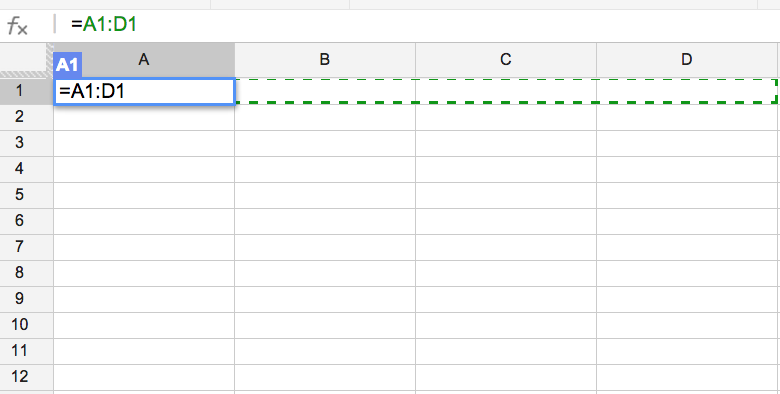
\includegraphics[width=1.0\textwidth]{images/03.png}}
  \begin{itemize}
      \item Если надо указать интервал, используется запись НАЧАЛО:КОНЕЦ.
      \item Начало --- верхний левый угол, конец --- правый нижний.
  \end{itemize}
\end{frame}

\subsection{Интервалы 2}
\begin{frame}[fragile]
  \frametitle{Интервалы}
  \centerline{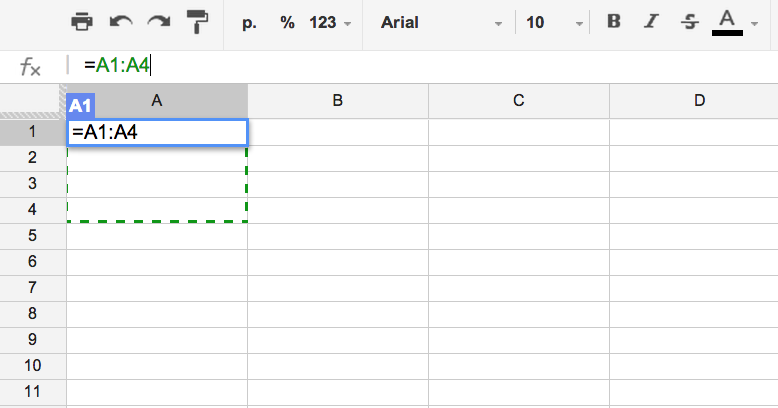
\includegraphics[width=1.0\textwidth]{images/02.png}}
\end{frame}

\subsection{Интервалы 3}
\begin{frame}[fragile]
  \frametitle{Интервалы}
  \centerline{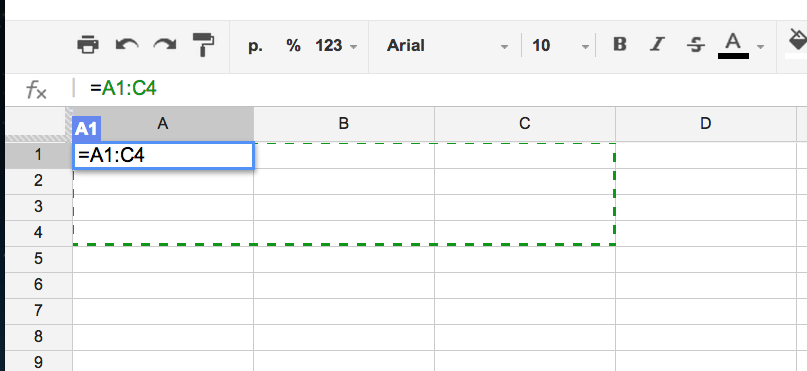
\includegraphics[width=1.0\textwidth]{images/01.png}}
\end{frame}

\subsection{Задача 1}
\begin{frame}[fragile]
  \frametitle{Интервалы}
  \centerline{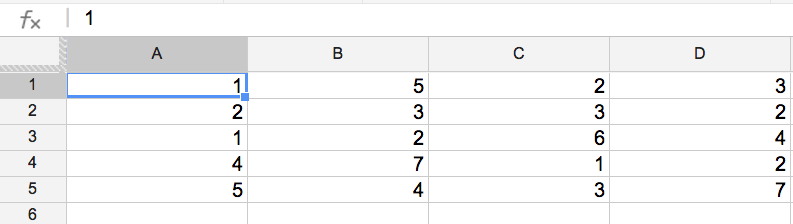
\includegraphics[width=1.0\textwidth]{images/04.png}}
  \begin{itemize}[<+->]
      \item Посчитать сумму элементов в интервалах:
      \item A1:A3
      \item A1:B2
      \item A2:C4
      \item C3:A2
  \end{itemize}
\end{frame}

\subsection{Задача 1}
\begin{frame}[fragile]
  \frametitle{Интервалы}
  \centerline{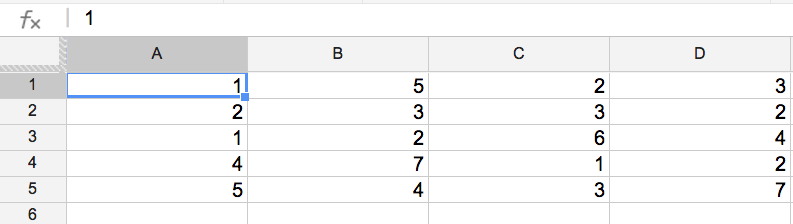
\includegraphics[width=1.0\textwidth]{images/04.png}}
  \begin{itemize}[<+->]
      \item Посчитать сумму элементов в интервалах:
      \item A1:A3 = 4
      \item A1:B2 = 11
      \item A2:C4 = 29
      \item C3:A2 = 17
  \end{itemize}
\end{frame}

\section{Функции}
\subsection{Функции}
\begin{frame}
  \begin{center}
    \Huge{Функции}
  \end{center}
\end{frame}

\subsection{Функции 2}
\begin{frame}[fragile]
  \frametitle{Функции}
  \begin{itemize}
    \item Если нужно провести какую-то стандартную операцию над интервалом, то можно использовать функции.
    \item Функции позволяют применить определённое действие ко всем ячейкам.
    \item Например, просуммировать значения.
    \item Или найти максимум / минимум.
    \item Или вычислить среднее значение.
    \item Функции отлично работают с огромным объёмом данных.
  \end{itemize}
\end{frame}

\subsection{Сумма}
\begin{frame}[fragile]
  \frametitle{Сумма}
  \centerline{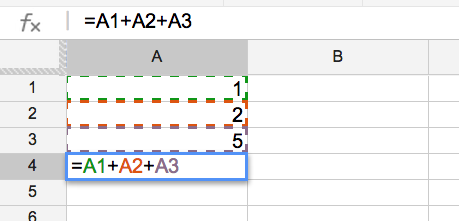
\includegraphics[width=1.0\textwidth]{images/06.png}}
  \begin{itemize}
      \item Допустим, надо найти сумму трёх ячеек.
      \item Можно делать, как сделано выше.
  \end{itemize}
\end{frame}

\subsection{Сумма облом}
\begin{frame}[fragile]
  \frametitle{А если так?}
  \centerline{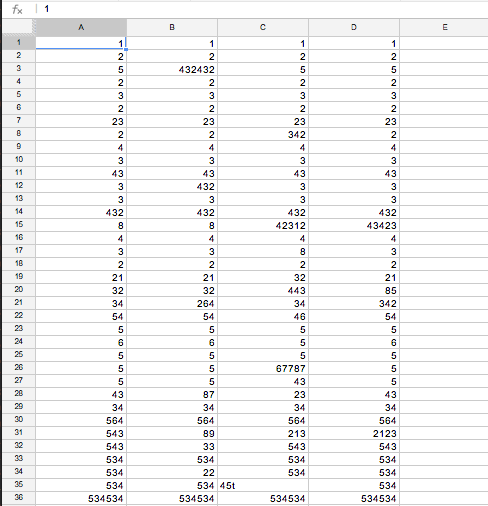
\includegraphics[width=0.5\textwidth]{images/07.png}}
\end{frame}

\subsection{Сумма 3}
\begin{frame}[fragile]
  \frametitle{ПААААНИКА!}
  \centerline{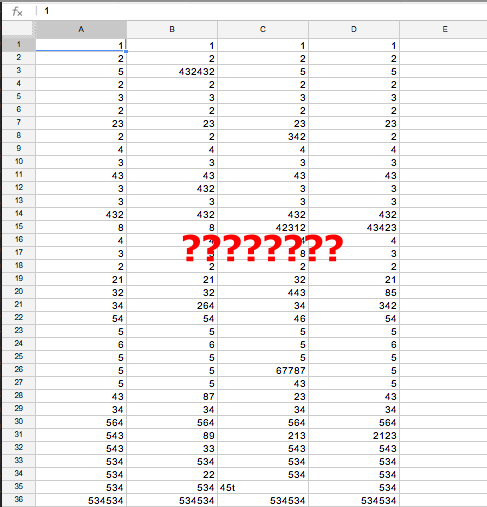
\includegraphics[width=0.5\textwidth]{images/07-2.png}}
\end{frame}

\subsection{Don't panic}
\begin{frame}[fragile]
  \frametitle{Don't panic}
  \centerline{
\includegraphics[width=0.8\textwidth]{images/dont_panic.jpg}}
\end{frame}

\subsection{SUM}
\begin{frame}[fragile]
  \frametitle{SUM}
  \centerline{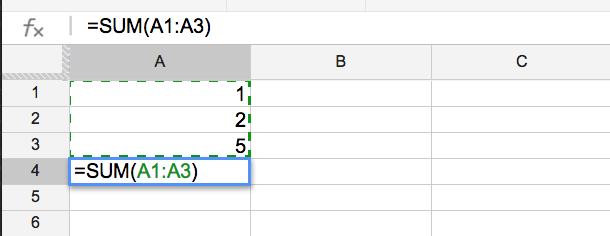
\includegraphics[width=1.0\textwidth]{images/05.png}}
  \begin{itemize}
      \item Функция SUM считает сумму по интервалу.
      \item =SUM(A1:A3)
  \end{itemize}
\end{frame}

\subsection{Автоподсказки}
\begin{frame}[fragile]
  \frametitle{Автоматические подсказки}
  \centerline{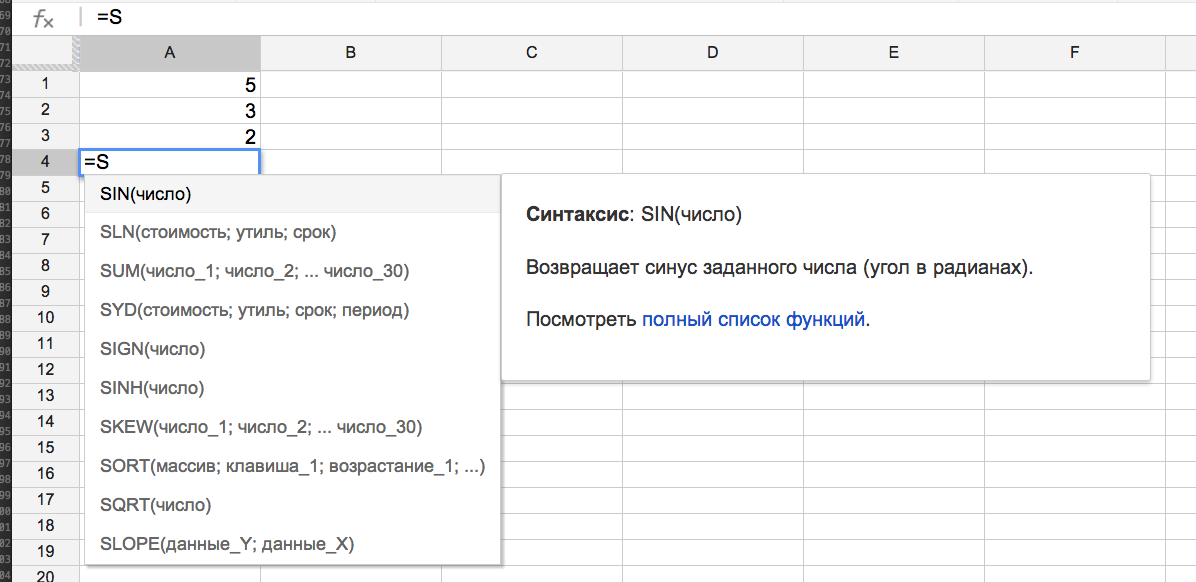
\includegraphics[width=0.9\textwidth]{images/09.png}}
  \begin{itemize}
      \item Просто введите = и первую букву --- программа сама подскажет.
      \item Количество функций --- 100500.
  \end{itemize}
\end{frame}

\subsection{Основные функции}
\begin{frame}[fragile]
  \frametitle{Основные функции}
  \begin{itemize}
    \item Список часто используемых функций:
  \end{itemize}
  \begin{tabular}{|l|l|l|}
      \hline
      Функция & Что делает & Пример \\
      \hline
      SUM & суммирует & =SUM(A1:A3) \\
      \hline
      AVERAGE & среднее арифметическое & =AVERAGE(A1:A3) \\
      \hline
      MAX & максимум в интервале & =MAX(A1:A3) \\
      \hline
      MIN & минимум в интервале & =MIN(A1:A3) \\
      \hline
      POWER & возводит в степень & =POWER(2;5) $2^5 = 32$ \\
      \hline
      SIN & находит синус радианах & =SIN(3.141592) \\
      \hline
      COS & находит косинус радианах & =COS(3.141592) \\
      \hline
      TODAY & сегодняшний день & =TODAY() \\
      \hline
  \end{tabular}
\end{frame}

\subsection{Подсказки 1}
\begin{frame}[fragile]
  \frametitle{Автоматические подсказки}
  \centerline{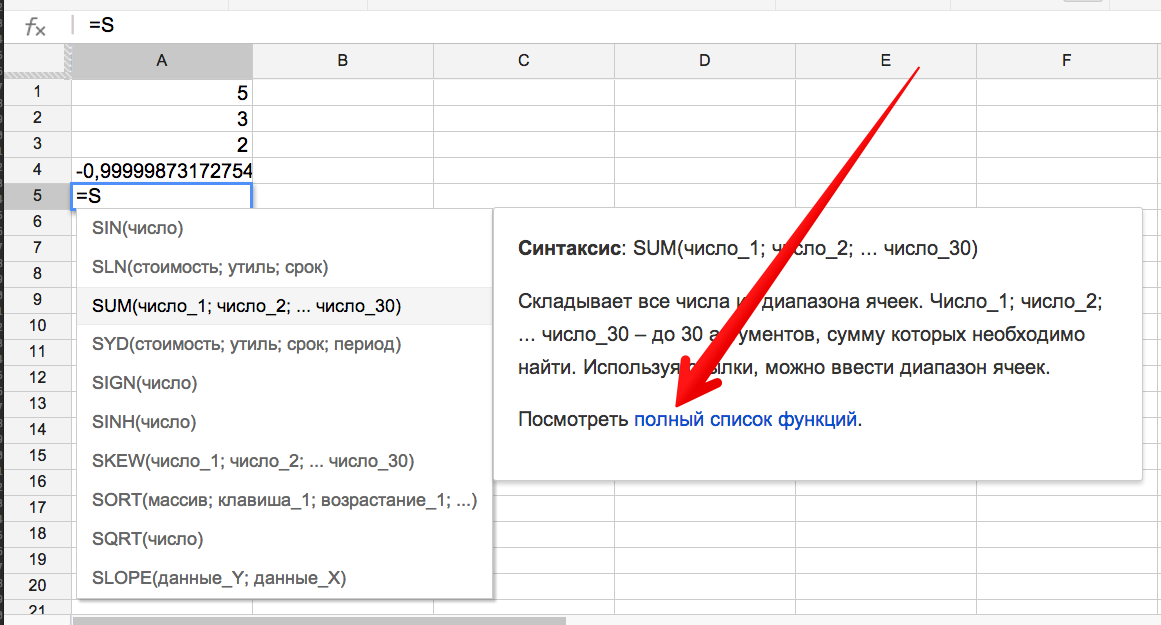
\includegraphics[width=0.9\textwidth]{images/10.png}}
  \begin{itemize}
      \item Список функций всегда легко ``подсмотреть''.
  \end{itemize}
\end{frame}

\subsection{Подсказки 2}
\begin{frame}[fragile]
  \frametitle{Автоматические подсказки}
  \centerline{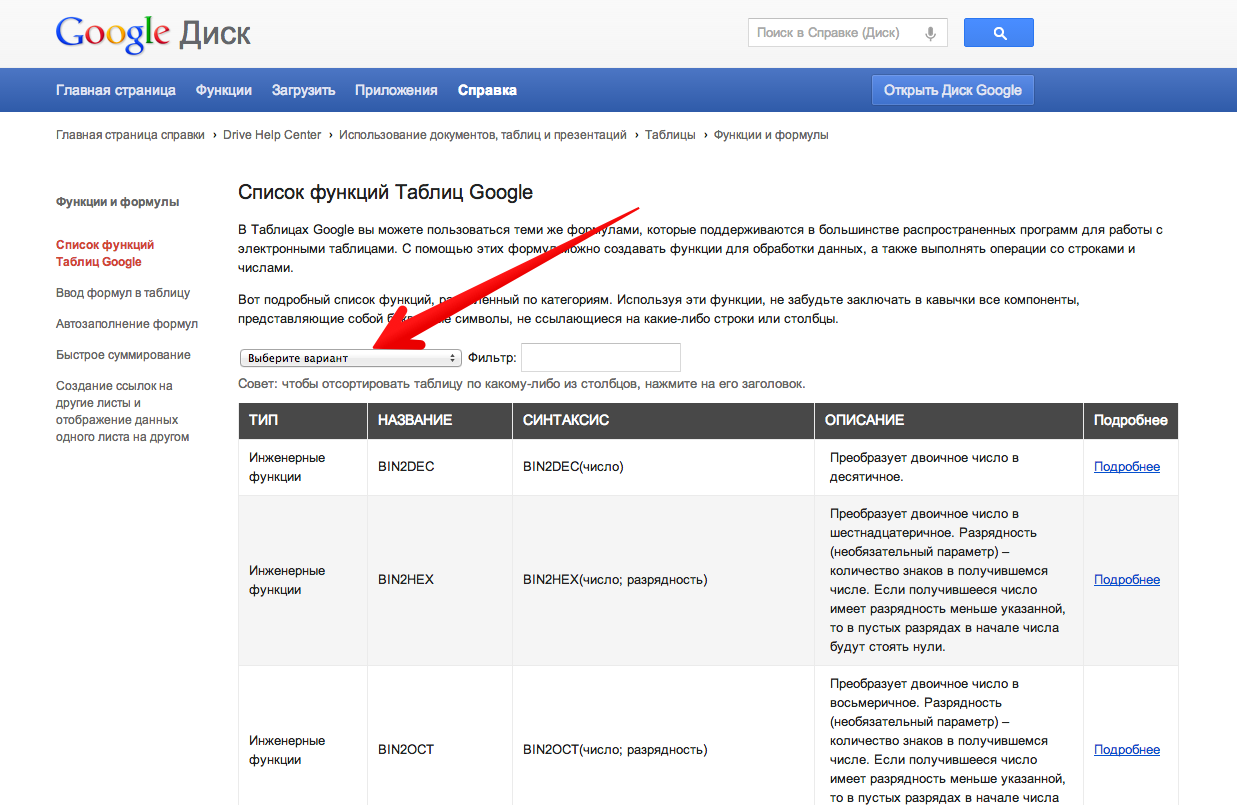
\includegraphics[width=0.9\textwidth]{images/10-2.png}}
  \begin{itemize}
      \item Список функций всегда легко ``подсмотреть''.
  \end{itemize}
\end{frame}

\subsection{Валюты}
\begin{frame}[fragile]
  \frametitle{Online}
  \begin{itemize}[<+->]
    \item А как насчёт валюты? Допустим, у меня есть 1000 долларов. Как узнать, сколько это в рублях сегодня?
    \item Хочется всего и автоматически.
    \item =GoogleFinance("CURRENCY:USDRUB")*1000
    \item А евро? Легко:
    \item =GoogleFinance("CURRENCY:EURRUB")*1000
    \item Google Drive позволяет автоматизировать всё!
  \end{itemize}
\end{frame}

\section{Задачи}

\subsection{Задачи}
\begin{frame}
  \begin{center}
    \Huge{Задачи}
  \end{center}
\end{frame}


\subsection{Задача 1.1}
\begin{frame}[fragile]
  \frametitle{Сумма}
  \centerline{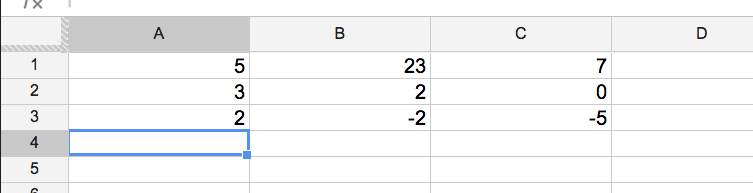
\includegraphics[width=1.0\textwidth]{images/11.png}}
  \begin{itemize}[<+->]
      \item =SUM(A1:B2)
      \item 33
  \end{itemize}
\end{frame}

\subsection{Задача 1.2}
\begin{frame}[fragile]
  \frametitle{Среднее}
  \centerline{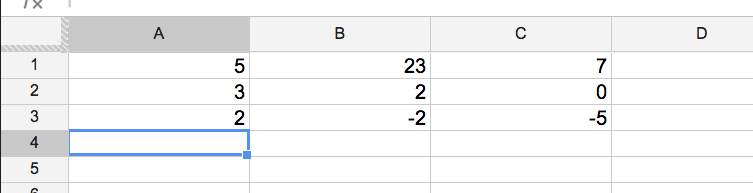
\includegraphics[width=1.0\textwidth]{images/11.png}}
  \begin{itemize}[<+->]
      \item =AVERAGE(B2:C3)
      \item -1.25
  \end{itemize}
\end{frame}

\subsection{Задача 1.3}
\begin{frame}[fragile]
  \frametitle{Максимум}
  \centerline{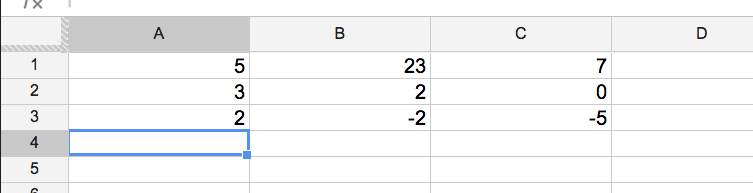
\includegraphics[width=1.0\textwidth]{images/11.png}}
  \begin{itemize}[<+->]
      \item =MAX(A1:C3)
      \item 23
  \end{itemize}
\end{frame}

\subsection{Задача 1.4}
\begin{frame}[fragile]
  \frametitle{Минимум}
  \centerline{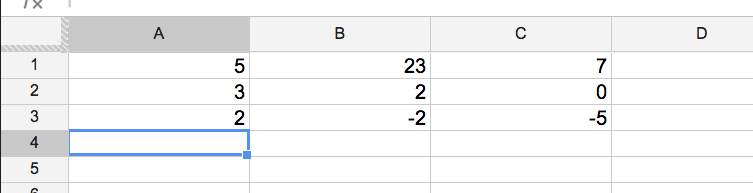
\includegraphics[width=1.0\textwidth]{images/11.png}}
  \begin{itemize}[<+->]
      \item =MIN(A1:C3)
      \item -5
  \end{itemize}
\end{frame}

\subsection{Задача 1.5}
\begin{frame}[fragile]
  \frametitle{Степень}
  \centerline{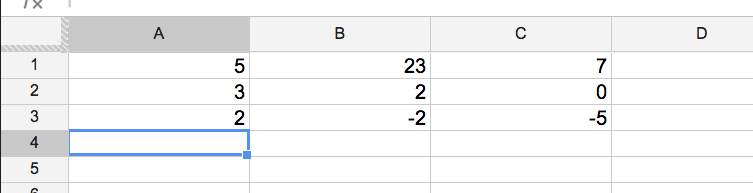
\includegraphics[width=1.0\textwidth]{images/11.png}}
  \begin{itemize}[<+->]
      \item =POWER(A3;10)
      \item 1024
  \end{itemize}
\end{frame}

\subsection{Задача 1.6}
\begin{frame}[fragile]
  \frametitle{Напоследок}
  \centerline{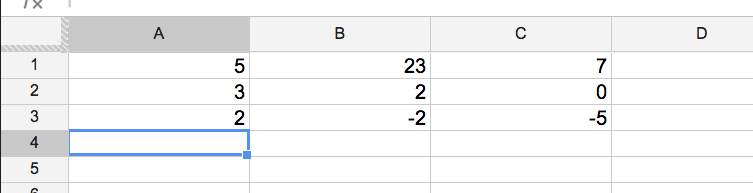
\includegraphics[width=1.0\textwidth]{images/11.png}}
  \begin{itemize}[<+->]
      \item =TODAY()
      \item 08.04.2013 (на момент составления презентации)
  \end{itemize}
\end{frame}

\subsection{Задача}
\begin{frame}[fragile]
  \frametitle{Задача}
  \begin{itemize}[<+->]
    \item \textbf{Задача.} Хочу узнать среднюю, максимальную и минимальную температуру за последние 2 недели в Санкт-Петербурге.
    \item Откуда брать данные?
    \item Много откуда. Например, http://gismeteo.ru.
    \item Итого, хочу таблицу: дата --- температура по всем датам. Затем автоматический подсчёт среднего, максимального и минимального значений.
  \end{itemize}
\end{frame}

\subsection{Задача 2}
\begin{frame}[fragile]
  \frametitle{Use the Force}
  \centerline{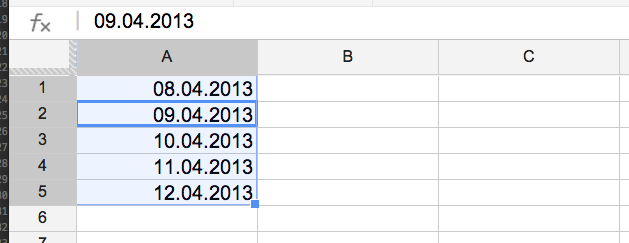
\includegraphics[width=1.0\textwidth]{images/12.png}}
  \begin{itemize}[<+->]
      \item Use the Force, Luke!
      \item Используйте магический синий квадратик, чтобы не вбивать даты вручную. Достаточно выделить два дня и потянуть за него.
  \end{itemize}
\end{frame}

\subsection{Задача 2 2}
\begin{frame}[fragile]
  \frametitle{Пример}
  \centerline{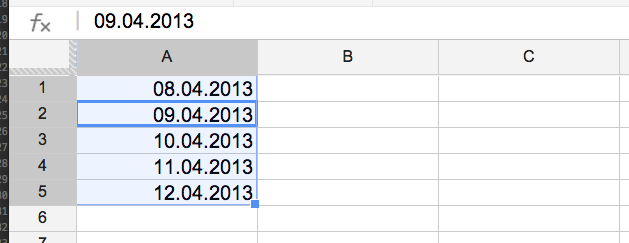
\includegraphics[width=1.0\textwidth]{images/12.png}}
  \begin{itemize}[<+->]
      \item Минимум и максимум считаем аналогично, подставляя MAX и MIN вместо AVERAGE.
  \end{itemize}
\end{frame}

\end{document}